\href{https://github.com/yassienE4/OS-VM/commit/9393c5952a805470bed9c5e1555c3382bce53cc0}{\ul{https://github.com/yassienE4/OS-VM/commit/9393c5952a805470bed9c5e1555c3382bce53cc0}}

How to run

\begin{itemize}
\item
  First make sure the python env is activated
\item
  ``source /workspaces/OS-VM/venv/bin/activate''
\item
  Second move to working directory
\item
  cd /workspaces/OS-VM/scheduling
\item
  ./run.sh main.cpp
\item
  ./main \textless directory\textgreater{}
  \textless bin\_width\textgreater{}
\item
  The c++ code should automatically call the python plot script
\end{itemize}

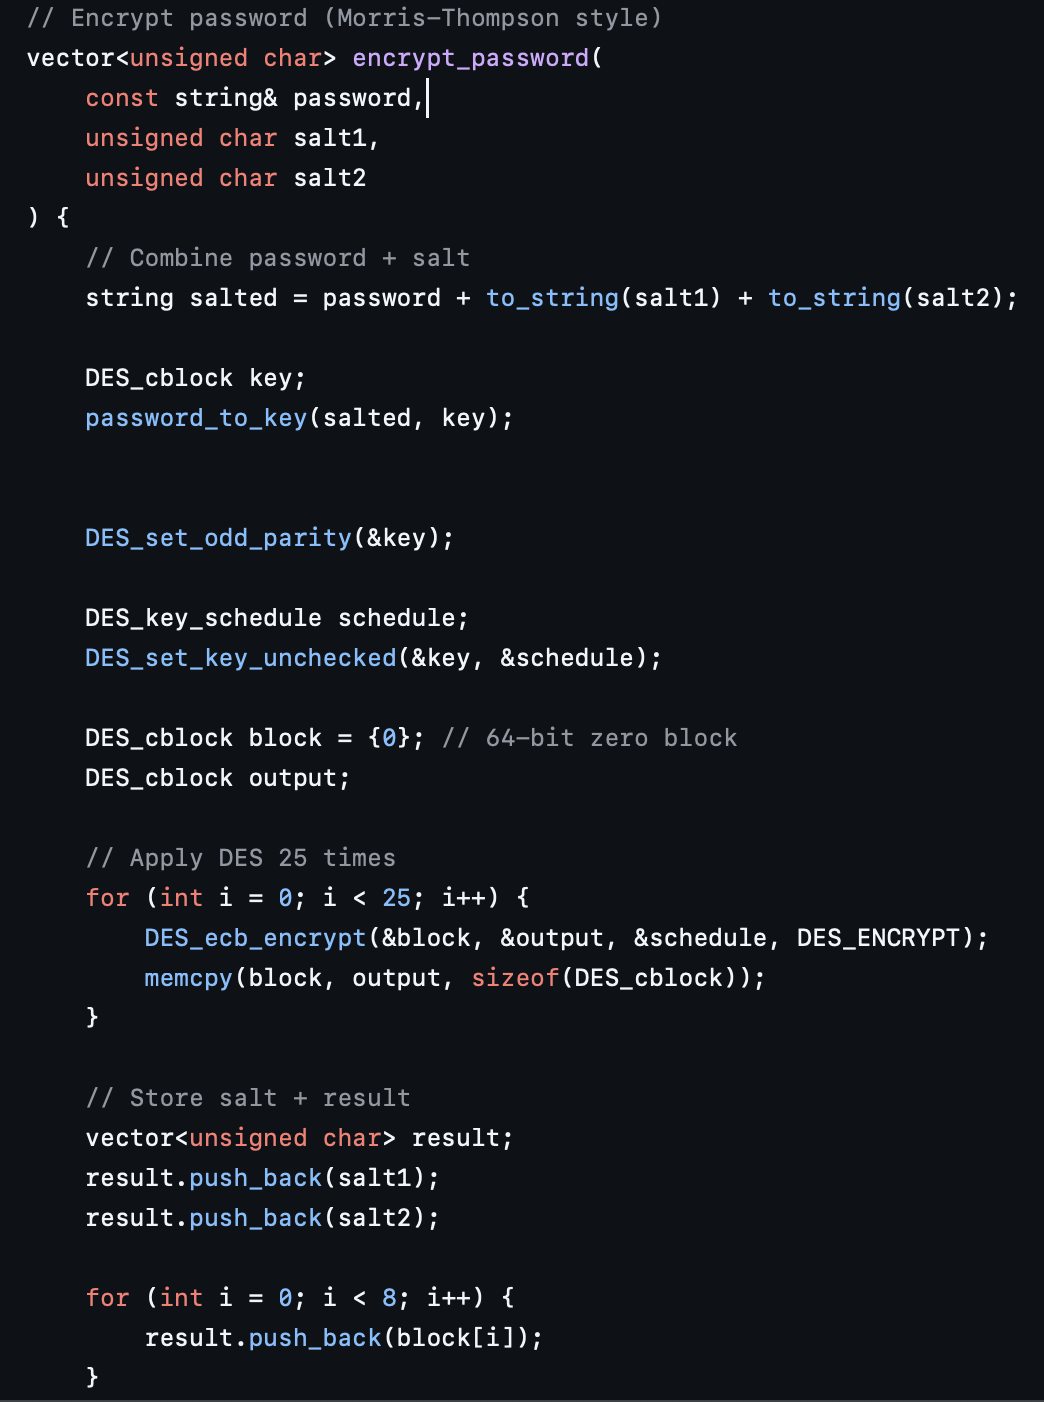
\includegraphics[width=6.5in,height=5.98611in]{./images/media/image4.png}

I represented the histogram as a map, Key = bin index, Value = number of
files in that bin

I used the library function recursive\_directory\_iterator to traverse
the file tree, calculated the filesize of each file and added it to the
map

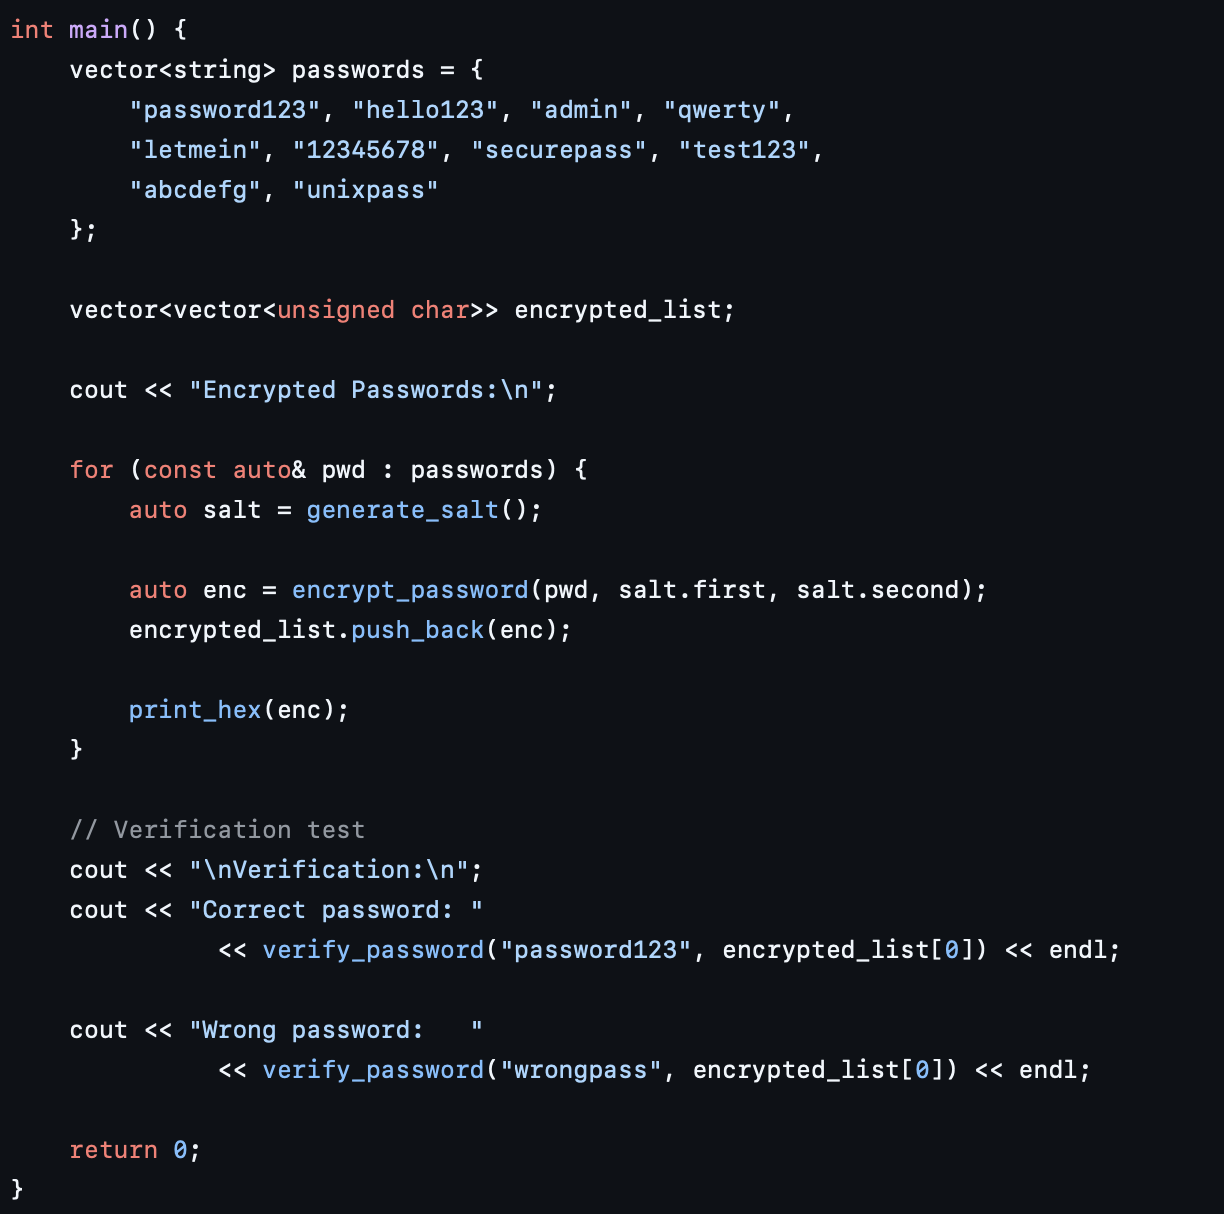
\includegraphics[width=4.46165in,height=3.68229in]{./images/media/image3.png}

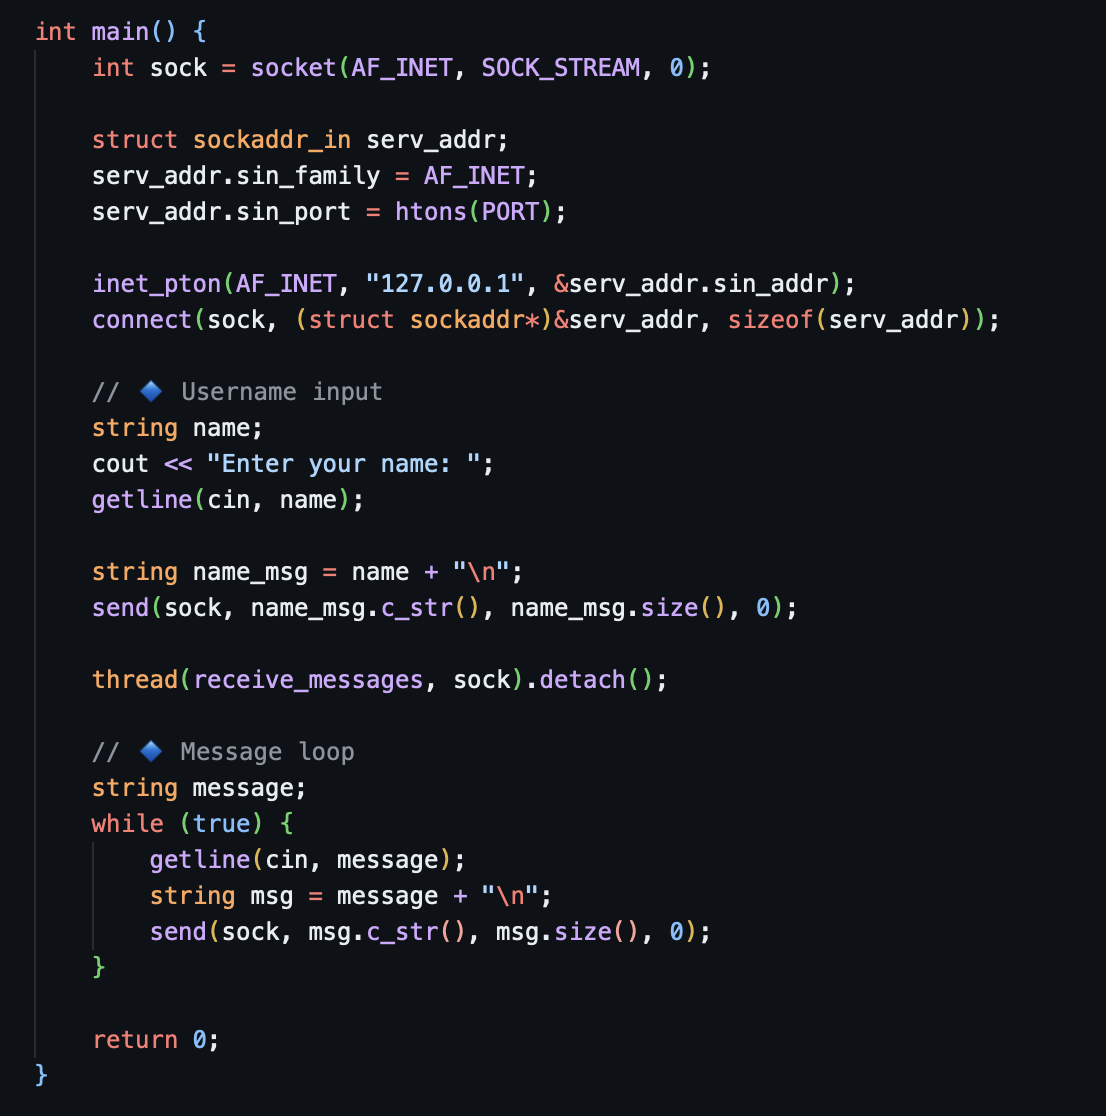
\includegraphics[width=3.96846in,height=3.82148in]{./images/media/image5.png}

To plot the histogram I first export the map as a CSV file which is then
read by a python file and using matplotlib I created a histogram and
saved it as a PNG.

Findings:

I ran ./main .. 1024\\
To look at the entire codespaces directory, with 1024 bin sizes

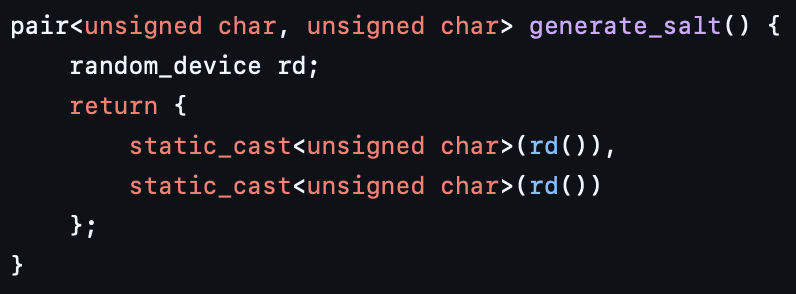
\includegraphics[width=3.82813in,height=4.66246in]{./images/media/image1.png}

As you can see there was a greater amount of smaller files then larger

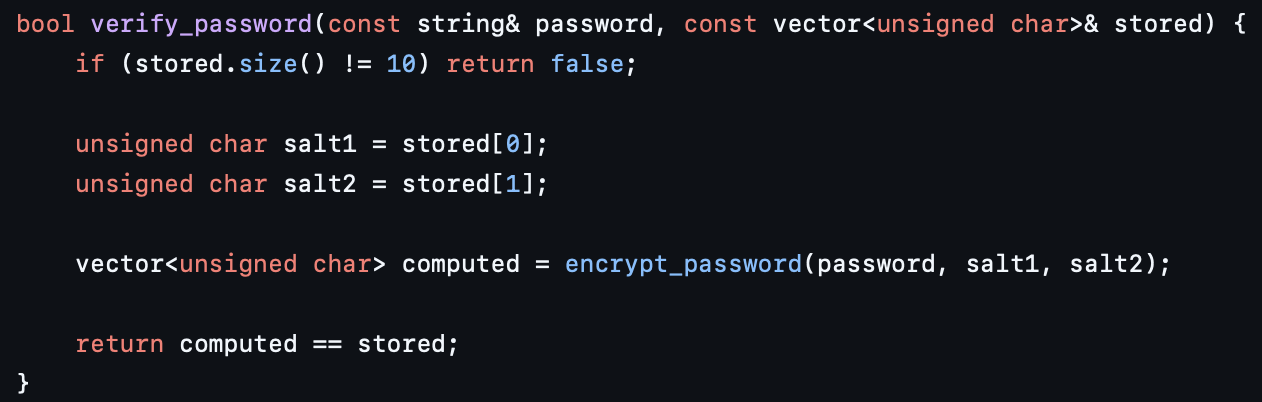
\includegraphics[width=3.80729in,height=2.85547in]{./images/media/image2.png}

Which is also represented in the histogram
